\subsection{Mouse spike data in an ethological foraging assay}
\label{subsection:aeon_results}

Unlike the linear track and trial-structured reaching tasks in \hyperref[subsection:synthetic_results]{\ref*{subsection:synthetic_results}} \& \hyperref[subsection:churchland_results]{\ref*{subsection:churchland_results}}, naturalistic behavior unfolds continuously over extended periods without predefined boundaries. We ask whether NLDisco can support open-ended feature discovery in this setting using Aeon, a platform for continuously recording rodent neural and behavioral activity in naturalistic habitats~\citep{campagner_2025_aeon_platform}. 

% This provides an opportunity to generate feature hypotheses from extended, unconstrained activity rather than limiting interpretation to experimenter-defined task conditions.

We analyze an 18-hour interval from a week-long Aeon experiment in which one mouse in an open environment spontaneously forages by spinning a wheel on a foraging patch (\autoref{figure:task_overview}c). The neural data come from a Neuropixels recording, processed into 20-ms binned spike counts from $N=90$ uncurated Kilosort units across retrosplenial cortex (RSC) and superior colliculus (SC). The behavioral data include the animal's centroid position and segmented image area estimated continuously from an overhead camera, together with foraging-wheel rotation and food-delivery events, with food dispensed every 75 cm of wheel movement (approximately three revolutions).

As before, we train a two-level Matryoshka TW-SED ($S = 20$, $(D_1,k_1)=(96,6)$, $(D_2,k_2)=(192,12)$, $B = 1024$) to reconstruct the neural data. Among many features found (see \hyperref[subsubsection:aeon_results_additional]{\ref*{subsubsection:aeon_results_additional}}), here we show one descriptive example, latent 52, surprisingly preferentially active for \textit{wheel activity}: wheel speeds $>$ 0.75 cm/s, $\metric{Sel}=0.839$, $\metric{AUROC}=0.924$ (\autoref{fig:aeon_features}). The preference persists when controlling for the animal's position, and notably, this association re-emerges across foraging bouts separated by hours: the same latent tracks wheel activity throughout the 18-hour recording (\autoref{fig:aeon_wheel_vs_patch}). Although RSC and SC are implicated in foraging, that did not predict the surprising wheel-associated feature revealed here. These associations suggest follow-up experiments, for example, varying wheel engagement while measuring posture and controlling location could help distinguish wheel-related activity from accompanying movements.

The interpretations also transfer across sessions. Keeping this model frozen and fitting only a new input mapping and decoder, initialised by matching units on probe position, to each of three further, separately spike-sorted sessions from adjacent days, without behavioral labels, latent 52 again tracks wheel activity in every session ($\metric{AUROC}=0.893$, $0.924$, and $0.913$, each the highest of the 192 shared latents). The latents for three supplementary features (segmented area, speed, and movement direction) of the $D=256$ model likewise rank first for their feature in all three sessions ($\metric{AUROC}$ $0.756$--$0.876$). When each model is retrained on 80\% of its recording and each feature's latent is chosen on that part alone, all eight features from \hyperref[subsection:churchland_results]{\ref*{subsection:churchland_results}} and this section keep their $\metric{Sel}$ and $\metric{AUROC}$ on the held-out 20\% (\hyperref[subsubsection:rebuttal_heldout]{\ref*{subsubsection:rebuttal_heldout}}). Even without training on a new session, zero-shot transfer by matching units across sessions by probe position preserves these interpretations: all four latents rank first for their features in each session (\hyperref[subsubsection:rebuttal_multisession]{\ref*{subsubsection:rebuttal_multisession}}). Beyond learning behavioral features, we find that NLDisco can also learn representations corresponding to environmental features: latents of a separate NLDisco model trained without stimulus labels on mouse visual cortex recordings~\citep{siegle_2021_allen_datasets} encode Gabor position, grating temporal frequency, and specific natural images and movie segments, with held-out $\metric{AUROC}$ of $0.770$--$0.972$ (\hyperref[subsubsection:rebuttal_allen_stimulus_features]{\ref*{subsubsection:rebuttal_allen_stimulus_features}}).

Last, we compare end-to-end feature discovery between NLDisco and the LVMs from \hyperref[subsection:churchland_results]{\ref*{subsection:churchland_results}} through two approaches, each using a common inspection budget, interpretation criterion, and held-out validation data. First, we ask how many prespecified behavioral features, defined before inspecting the models, can be recovered in individual latents: NLDisco, ST-NDT, and PCA each recover 5 of 12, CEBRA-Time recovers 2, and LangevinFlow recovers none. Second, to assess open-ended discovery, blinded AI agent raters interpret 32 randomly drawn latents per method; held-out validation supports interpretations for 33\% of NLDisco latents, 16\% of CEBRA-Time, 6\% of ST-NDT, 2\% of PCA, and none of LangevinFlow (\hyperref[subsubsection:rebuttal_discovery_comparison]{\ref*{subsubsection:rebuttal_discovery_comparison}}).

\begin{figure}[tb]
    \centering
    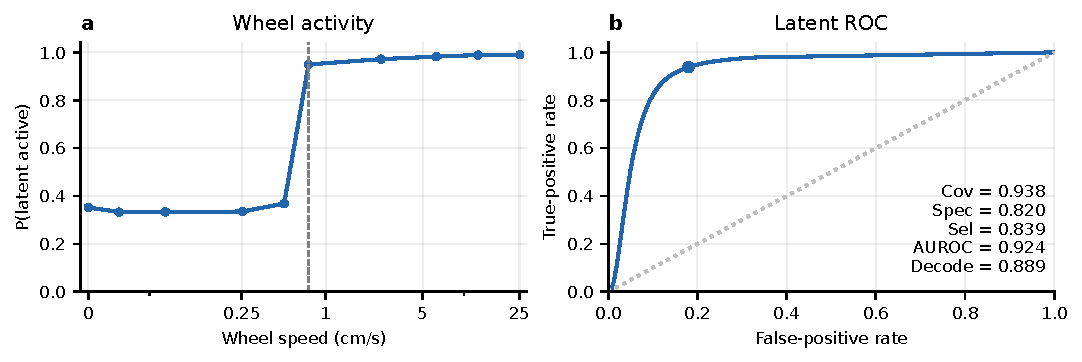
\includegraphics[width=\linewidth]{figures/aeon_main.pdf}
    \caption{\textbf{A \textit{wheel activity} latent in a continuous foraging recording.} (\textbf{a}) Latent activation probability by wheel speed; vertical dashed line at 0.75 cm/s. (\textbf{b}) ROC based on latent activations; dot: FPR 0.180, TPR 0.938 at the displayed activation threshold. \metric{Decode}: test balanced accuracy of a single-latent logistic decoder with a validation-selected decision threshold (\hyperref[paragraph:latent_decoding]{\ref*{subsubsection:latents_evaluation_details}}). Source activity traceback appears in \autoref{fig:aeon_wheel_source_traceback}.}
    \label{fig:aeon_features}
\end{figure}
